\section{Virtualios mašinos aprašas}

\subsection{Virtualios mašinos samprata}

Virtuali mašina – tai virtuali realios mašinos kopija. Virtuali reiškia netikra. Į virtualią mašiną surenkame reikalingas realios mašinos komponentes, tokias kaip procesorius, atmintis, įvedimo/išvedimo įrenginiai, suteikiame jiems paprastesnę nei reali vartotojo sąsaja ir visa tai pavadiname virtualia mašina.

\subsection{Virtualios mašinos komponentų aprašymas}
\begin{description}
\item[Atmintis] \leavevmode 

Virtualios mašinos (VM) atmintis sudaryta iš 16 žodžių po 4 baitus. 10 žodžių sudarys bloką. Kiekvienai VM skiriama po 10 blokų. Tuose dvidešimtyje blokų turi tilpti programa.
Pirmuose trijuose blokuose bus saugomos programos komandos, o likusiuose septyniuose – programos darbui reikalingi duomenys.
Ryšiai tarp realaus ir virtualaus adreso bus nusakomi per puslapiavimo mechanizmą. Puslapiavimo lentelė bus saugoma paskutiniuose penkiuose atminties blokuose.


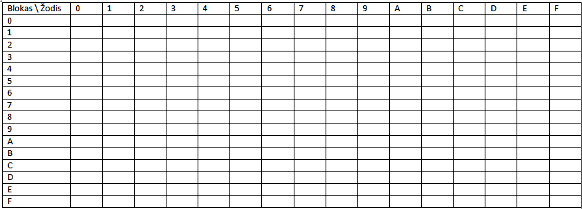
\includegraphics{VMatmintis.PNG}

\item[Procesorius]  \leavevmode 
  
VM procesorius turės vieną duomenų registrą, tris segmentų registrus, du nuorodų registrus bei du loginius registrus.
\begin{enumerate}
\item Duomenų registras:\leavevmode \\
DR – Data Register – naudojamas duomenų (žodžių) pakrovimui į jį iš atminties ir iš jo į atmintį. Taip pat operacijose.
\item Segmentų registrai:\leavevmode \\
CS – Code Segment – rodyklė į kodo segmentą atmintyje.\\
DS – Data Segment – rodyklė į duomenų segmentą atmintyje.\\
ST – Stack Segment – rodyklė į steko segmentą atmintyje.
\item Nuorodų registrai:\leavevmode \\
PC – Program Counter – jame saugomas einamosios komandos žodžio indeksas.\\
SP – jame saugomas steko viršūnės žodžio indeksas.
\item Loginiai registrai:\leavevmode \\
SF – Status Flag – pagal palyginimo operacijos rezultatą jis įgyja reikšmes:  \\ 0 – jei daugiau,\\ 1 – jei lygu, \\2 – jei mažiau.\\
DF – Data Format – pagal iš atminties nuskaityto žodžio duomenų formatą jis įgyja reikšmes: \\0 – nuskaitytas žodis kaip simboliai,\\ 1 – nuskatytas žodis kaip sveikas skaičius su ženklu.
\end{enumerate}  
\item[Komandų sistema] \leavevmode 
\begin{enumerate}
\item Aritmetinės komandos: \leavevmode 
\begin{itemize}
\item ADD – sudeda du viršutinius steko elementus, sumažina steko rodyklę SP vienetu ir padeda rezultatą į steko viršūnę.\leavevmode 
\\ST [SP – 1] = ST [SP – 1] + ST [SP]; \\SP--;\\
\item SUB – atima steko viršūnėje esantį elementą iš antro nuo viršaus steko elemento, steko rodyklę SP sumažina vienetu bei rezultatą priskiria steko viršūnei.\leavevmode
\\ST [SP – 1] = ST [SP – 1] – ST [SP] ; \\SP--;\\
\item MUL – sudaugina du viršutinius steko elementus, sumažina steko rodyklę SP vienetu ir padeda rezultatą į steko viršūnę.\leavevmode
\\ST [SP – 1] = ST [SP – 1] * ST [SP]; \\SP--;\\
\item DIV – padalina antrą nuo viršaus steko elementą iš viršūnėje esančiojo, sumažina SP vienetu ir padeda rezultatą į steko viršūnę.\leavevmode
\\ST [SP – 1] = ST [SP – 1] / ST [SP]; \\SP--;\\
\item NEG – registre DR esantį žodį pakeičia jam priešingu.\leavevmode
\\DR = 0 – DR;\\
\end{itemize}
\item Logikos operacijų bitinės komandos:
\begin{itemize}
\item AND – atlieka dviejų viršutinių steko elementų konjunkciją, SP sumažina vienetu ir rezultatą priskiria steko viršūnei. \leavevmode
\\ST [SP – 1] = ST [SP – 1]  \& ST [SP];\\ SP--;\\
\item OR – atlieka dviejų viršutinių steko elementų disjunkciją, SP sumažina vienetu ir rezultatą priskiria steko viršūnei. \leavevmode
\\ST [SP – 1] = ST [SP – 1] ¦ ST [SP];\\ SP--;\\
\item NOT – atlieka registre DR esančio žodžio loginį neigimą (inversiją). \leavevmode
\\DR = !(DR);\\
\end{itemize}
\item Palyginimo komanda:
\begin{itemize}
\item CMP – ši komanda palygina registre DR esantį žodį su steko viršūnėje esančiu žodžiu ir pagal palyginimo rezultatą formuoja registro SF reikšmę: \leavevmode
\\0 – jei DR > ST [SP], 
\\1 – jei DR = ST [SP],
\\ 2 – jei DR < ST [SP].
\end{itemize}
\item Darbo su duomenimis komandos:
\begin{itemize}
\item LBxy – į registrą DR užkrauna žodį iš duomenų segmento nurodytu adresu 10*x + y bei formuoja DF = 0 požymį, reiškiantį, kad registre DR – simbolinė informacija.\\
\item LWxy – į registrą DR užkrauna žodį iš duomenų segmento nurodytu adresu 10*x + y bei formuoja DF = 1 požymį, reškiantį, kad registre DR – sveikas skaičius su ženklu.\\
\item SWxy – registre DR esantį žodį, nepriklausomai nuo to ar tai simbolinė, ar skaitinė informacija, dedame į duomenų segmentą nurodytu adresu 10*x + y.\\
\end{itemize}
\item Steko operacijos:
\begin{itemize}
\item PUSH – steko viršūnė SP padidinama vienetu ir į ja patalpinamas registre DR esantis žodis.\leavevmode
\\SP = SP + 1; \\ST [SP] = DR;
\item POP – steko viršūnėje esantis žodis talpinamas į registrą DR ir SP sumažinama vienemtu.\leavevmode
\\DR = ST [SP];\\ SP--;
\end{itemize}
\item Valdymo komandos:
\begin{itemize}
\item JMxy – nesąlyginio valdymo perdavimo komanda. Ji reiškia, kad valdymas turi būti perduotas kodo segmento žodžiui, nurodytam adresu 10*x + y.\leavevmode
\\PC = 10*x + y;
\item JLxy – jeigu SF = 2, tai valdymas perduodamas nurodytu adresu 10*x + y.\leavevmode
\\If (SF = 2)\\ PC = 10*x + y;
\item JExy – jeigu SF = 1, tai valdymas perduodamas nurodytu adresu 10*x + y.\leavevmode
\\If (SF = 1)\\PC = 10*x + y;
\item HALT – programos sustojimo taško komanda.
\end{itemize}
\item Įvedimo/Išvedimo komandos:
\begin{itemize}
\item PDRB – registre DR esantį žodį traktuoja kaip keturis baitus, t.y. keturis simbolius ir juos išveda išvedimo įrenginį.\leavevmode
\item PDRW – registre DR esantį žodį traktuoja kaip skaitinę informaciją ir išveda skaičių į išvedimo Įrenginį.\leavevmode
\end{itemize}
 \end{enumerate}

\end{description}   
   
\subsection{Virtualios mašinos bendravimo su įvedimo/išvedimo įrenginiais
mechanizmo aprašymas}

\subsection{Virtualios mašinos interpretuojamojo vykdomojo failo išeities 
teksto formatas}

Užduoties kodas yra surašomas faile. Visame faile rašant tik vykdymui reikalingas
komandas. Paskutinė vykdoma komanda privalo būti HALT. Kitu atveju virtualios mašinos darbo
rezultatai nėra apibrėžti.

Bendra programos schema:\\
\\\textbf{DATASEG:}

DW simbolinis žodis – 4simboliai tarp kabučių (pvz.: DW "ABCD")

DPI neneigiamas sveikas skaičius (pvz. DPI 5)

DNI neigiamas sveikas skaičius (pvz. DNI -2)
\\\textbf{CODESEG:}

<komandos po 4 simbolius>\\
\textbf{HALT}

\subsection{Modeliuojamos virtualios mašinos loginių komponentų sąryšio su 
realios mašinos techninės įrangos komponentais aprašymas}

   
%Visi skaičiai yra su ženklu!

%Komandų argumentai nurodyti 16-ainiais skaičiais.
